\thispagestyle{plain}
\chapter{ Αποτελέσματα και Μελλοντικές Επεκτάσεις}
\label{chap:7}



\section{Οπτικοποίηση με Grad-CAM}
\label{chap:7.1}

Η οπτικοποίηση των περιοχών που εστιάζει το νευρωνικό έχει διττό ρόλο στο πρόβλημα καθώς δίνει πληροφορίες για τη λειτουργία του νευρωνικού ενώ συγχρόνως αποτελεί ένα κατευθυντήριο μέσο για τον ιατρό στη διαδικασία της διάγνωσης, καθώς επισημαίνει τις περιοχές που βρίσκεται η ασθένεια. 


\subsection{Μέθοδος Grad-CAM} 
\label{sec:7.1.1}
Gradient class activation maps(Grad-CAM) είναι μία τεχνική οπτικοποίησης για τα βαθιά συνελικτικά δίκτυα \cite{Ramprasaath}. Παρακάτω παρουσιάζεται η διαδικασία που ακολουθείται μέχρι την τελική οπτικοποίηση.
Αρχικά, υπολογίζεται  η κλίση της πρόβλεψης $y^c$ της κλάσης c (πριν την εφαρμογή της συνάρτησης softmax), ως προς τους χάρτες χαρακτηριστικών $ A^k $ κάποιου συνελικτικού επιπέδου( $\frac{\partial y^c}{\partial A^k }$). Είναι δυνατόν να επιλεχθεί οποιοδήποτε συλλεκτικό επίπεδο, ωστόσο προτιμάτε το τελευταίο καθώς περιέχει την περισσότερη πληροφορία.
 Έπειτα, εφαρμόζεται καθολική υποδειγματοληψία για να υπολογιστούν τα βάρη $a_{k}^c$ για κάθε χάρτη χαρακτηριστικών. Το βάρος $a_{k}^c$   αποδίδει τη σημασία του k χάρτη χαρακτηριστικών για την κλάση c. Η παραπάνω διαδικασία αυτή παρουσιάζεται στην εξίσωση \ref{eq:7.10}.

\begin{equation} \label{eq:7.10}
a_{k}^c =  \frac{1}{Z} \sum_{i}  \sum_{j} \frac{\partial y^c}{\partial A_{ij}^k }
\end{equation}

Τέλος, ο κάθε χάρτης χαρακτηριστικών πολλαπλασιάζεται με το αντίστοιχο βάρος του και στη συνέχεια εφαρμόζεται συνάρτηση Ανόρθωσης. Επιλέγεται η εφαρμογή της συνάρτησης Ανόρθωσης γιατί χρήσιμα είναι τα χαρακτηριστικά που έχουν θετική επιρροή στην κλάση ενδιαφέροντος όπως εικονοστοιχεία  που η ένταση τους πρέπει να αυξηθεί για να αυξηθεί η $y^{c}$. Χωρίς τη συνάρτηση Ανόρθωσης είναι πολύ πιθανό να επισημανθούν στοιχεία άσχετα με την επιθυμητή κλάση.

\begin{equation} \label{eq:7.11}
L_{GradCAM}^c =  ReLU(\sum_{k} a_{k}^c  A^k)
\end{equation}

 Στην εικόνα \ref{fig:fm1} παρουσιάζονται κάποιοι από τους  χάρτες χαρακτηριστικών, για είσοδο μία τυχαία εικόνα του συνόλου ελέγχου ενός συνελικτικού επιπέδου 35x35 του νευρωνικού και στην \ref{fig:fm2}  κάποιοι από τους χάρτες χαρακτηριστικών του τελευταίου συνελικτικού επιπέδου 8x8 για την ίδια εικόνα. Είναι φανερό ότι οι χάρτες χαρακτηριστικών 35x35 δείχνουν με πολύ μεγαλύτερη ακρίβεια τις περιοχές ενεργοποίησης του μοντέλου ωστόσο οι χάρτες χαρακτηριστικών του τελευταίου συνελικτικού επιπέδου περιέχουν περισσότερη πληροφορία σχετικά με την ενεργοποίηση των κλάσεων. 




\begin{figure}[!h]
\centering
\begin{subfigure}{.5\textwidth}
  \centering
  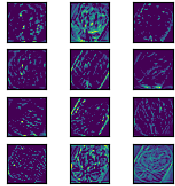
\includegraphics[scale=1.05]{f1.png}
  \caption{Χάρτες Χαρακτηριστικών 35x35}
  \label{fig:fm1}
\end{subfigure}
\begin{subfigure}{.5\textwidth}
  \centering
  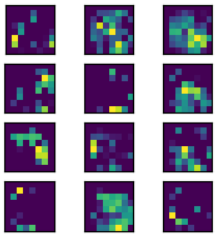
\includegraphics[scale=1]{f2.PNG}
  \caption{Χάρτες Χαρακτηριστικών 8x8}
  \label{fig:fm2}
\end{subfigure}
\caption{Όπτικοποίηση των Χαρτών Χαρακτηριστικών για μία τυχαία εικόνα του συνόλου ελέγχου}
\label{figure:fm}
\end{figure}




\subsection{ Αποτελέσματα οπτικοποίησης Νευρωνικού} 
\label{sec:7.1.3}

Όπως εξηγήθηκε και πιο πάνω οι περιοχές στις οποίες εστιάζει το νευρωνικό για να ταξινομήσει μια εικόνα στην κλάση rDR, εξάγονται από χάρτες χαρακτηριστικών διαστάσεων $8x8$. H παραπάνω μέθοδος μετά τη διαδικασία που εξηγήθηκε παραπάνω παράγει μία εικόνα διαστάσεων $8x8$, η οποία περιέχει τις περιοχές ενεργοποίησης της κλάσης rDR.
Έτσι, όταν γίνεται υπερδειγματοληψία στην  $8x8$ εικόνα, για αύξηση των διαστάσεων της εικόνας σε $299x299$, μία περιοχή 8x8 στην αρχική εικόνα, θα αντιστοιχίζεται σε μια περιοχή 37x37 στην νέα εικόνα. Με την παραπάνω ανάλυση γίνεται φανερό το πρόβλημα που αντιμετωπίζει η μέθοδος στον ακριβή προσδιορισμό των περιοχών της ασθένειας. 

Όπως θα γίνει φανερό και από τα παραδείγματα που θα παρουσιαστούν παρακάτω, οι περιοχές ενδιαφέροντος συνήθως εντοπίζονται σε μεγαλύτερη επιφάνεια από τα πραγματικά συμπτώματα. Επιπλέον, περιοχές που υπάρχουν πολλά συμπτώματα, παρουσιάζονται στην εικόνα ως μία ενιαία μεγάλη περιοχή. Τέλος, λόγω  της μικρής διάστασης των χαρτών χαρακτηριστικών, κάποιες φορές στις περιοχές ενεργοποίησης περιλαμβάνεται και το φόντο της εικόνας. Παρακάτω, θα σχολιαστούν κάποια παραδείγματα οπτικοποίησης.

Για τη γραφική αναπαράσταση των περιοχών ενδιαφέροντος έγινε χρήση Heat map. Ουσιαστικά, οι περιοχές ενδιαφέροντος εντοπίζονται με επίκεντρο στο πορτοκαλί χρώμα και φθίνουν μέχρι το κυανό. Οι περιοχές με μπλε χρώμα θεωρούνται μη σημαντικές για την ταξινόμηση στην κλάση rDR.

Στην εικόνα \ref{figure:viz1n} παρατηρούνται μία πληθώρα συμπτωμάτων, τα οποία ανιχνεύει το μοντέλο. Μεγαλύτερη βάση δίνεται στην περιοχή με πιο έντονα τα συμπτώματα της ασθένειας, η οποία χρωματίζεται με πορτοκαλί. Μεγάλη επιφάνεια καταλαμβάνει το κυανό χρώμα που αποτελεί σημείο ενδιαφέροντος, ωστόσο με μικρότερη  επιρροή για την τελική απόφαση αφού στην περιοχή αυτή υπάρχουν κάποια διάσπαρτα εξιδρώματα ενώ στον οπτικό δίσκο παρατηρείται ανάπτυξη νέων αγγείων.

Στην εικόνα \ref{figure:viz2n} τα χαρακτηριστικά είναι πολύ πιο ήπια για τον παρατηρητή ωστόσο το νευρωνικό ανιχνεύει 3 περιοχές ενδιαφέροντος, που περιέχουν βαμβακόμορφες κηλίδες και ίσως κάποια νεοαγγεία. Στη συγκεκριμένη εικόνα γίνεται φανερό ότι το μοντέλο μπορεί και εντοπίζει και πιο ήπια συμπτώματα που δεν καταλαμβάνουν πολύ χώρο.

Στην εικόνα \ref{figure:viz3n} υπάρχει μία περιοχή με πολλά σκληρά εξιδρώματα την οποία εντοπίζει το νευρωνικό. Στη περιοχή αυτή φαίνονται πολύ έντονα τα εξιδρώματα τα οποία αποτελούν κύριο σύμπτωμα της ασθένειας ωστόσο εξιδρώματα απαντώνται σε όλη την εικόνα σε ηπιότερη μορφή . Το νευρωνικό μπορεί να έχει ανιχνεύσει και αυτές τις περιοχές ωστόσο η επιρροή τους για την τελική απόφαση να είναι αμυδρή σε σχέση με την επιρροή της μεγάλης περιοχής και για αυτό να μην αναπαριστάται στο Heatmap. 

Η εικόνα \ref{figure:viz4n} επισημαίνονται δύο ενωμένες περιοχές ενδιαφέροντος με τη μία πάνω και δεξιά από τον οπτικό δίσκο και την άλλη κάτω και δεξιά. Η πάνω και δεξιά περιοχή περιλαμβάνει μία  βαμβακόμορφη κηλίδα ενώ στην κάτω δεξιά εντοπίζεται μια  βαμβακόμορφη κηλίδα μεγαλύτερων διαστάσεων και ένα αιμάτωμα. Στην οπτικοποίηση επισημαίνεται με πιο έντονο χρωματισμό ότι η κάτω περιοχή αποτελεί πιο έντονο σύμπτωμα της ασθένειας καθώς η  βαμβακόμορφη κηλίδα καταλαμβάνει μεγαλύτερη επιφάνεια.


%\begin{figure}[!h]
%    \centering
%      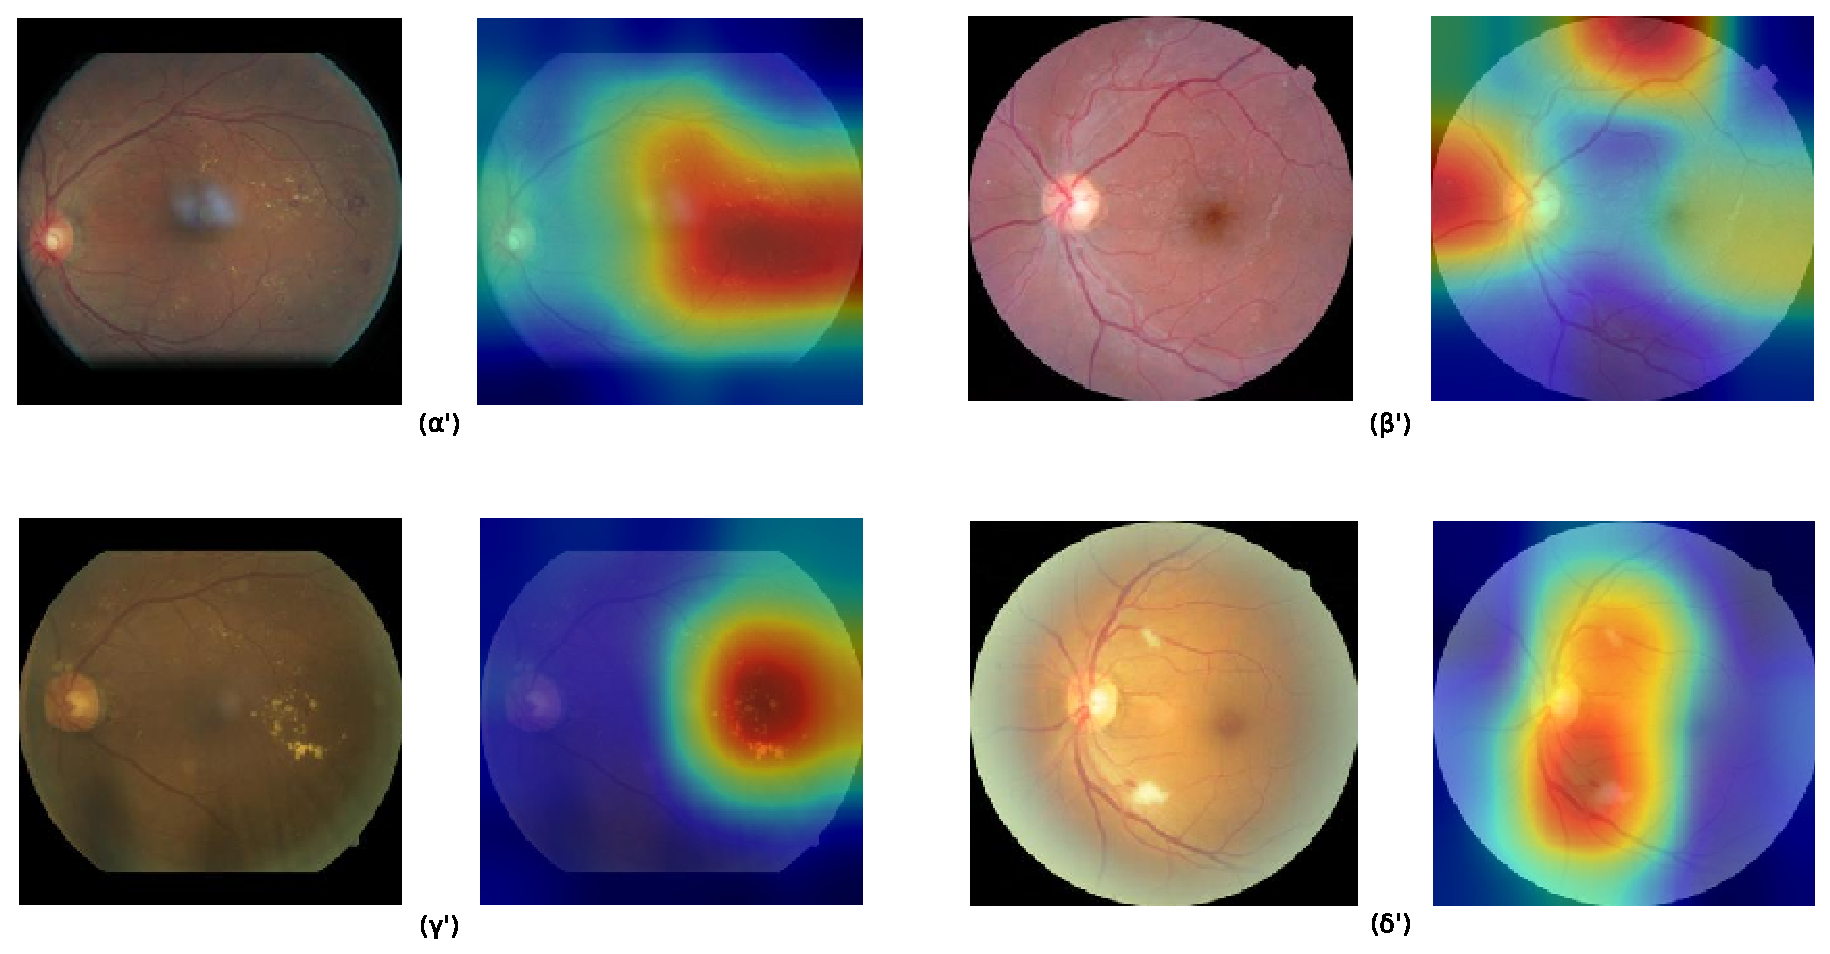
\includegraphics[width=1\linewidth]{vis.pdf} %\caption{Οπτικοποίηση των περιοχών με DR}
%      \label{figure:viz}    
%  \end{figure}


\begin{figure}[!h]
    \centering
      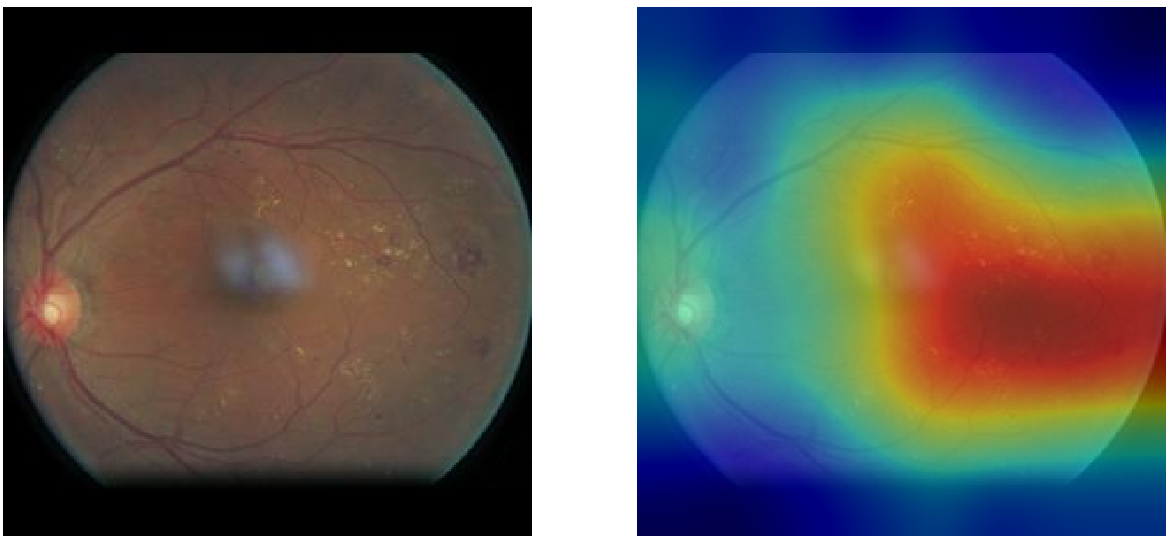
\includegraphics[width=0.75\linewidth]{1.png} \caption{Οπτικοποίηση των περιοχών με DR - Δείγμα 1}
      \label{figure:viz1n}    
  \end{figure}

\begin{figure}[!h]
    \centering
      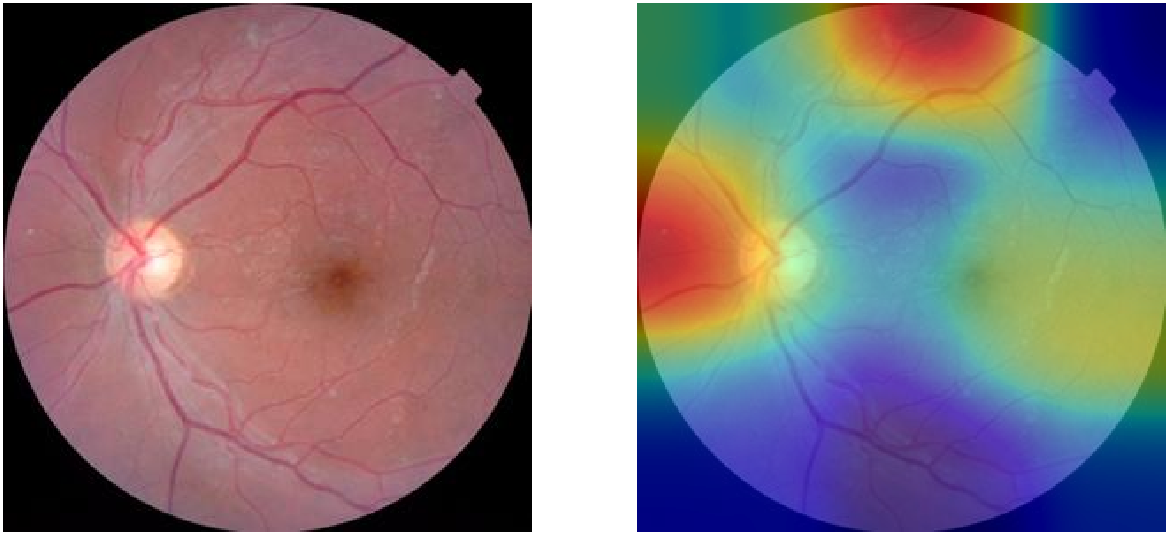
\includegraphics[width=0.75\linewidth]{2.png} \caption{Οπτικοποίηση των περιοχών με DR - Δείγμα 2}
      \label{figure:viz2n}    
  \end{figure}

\begin{figure}[!h]
    \centering
      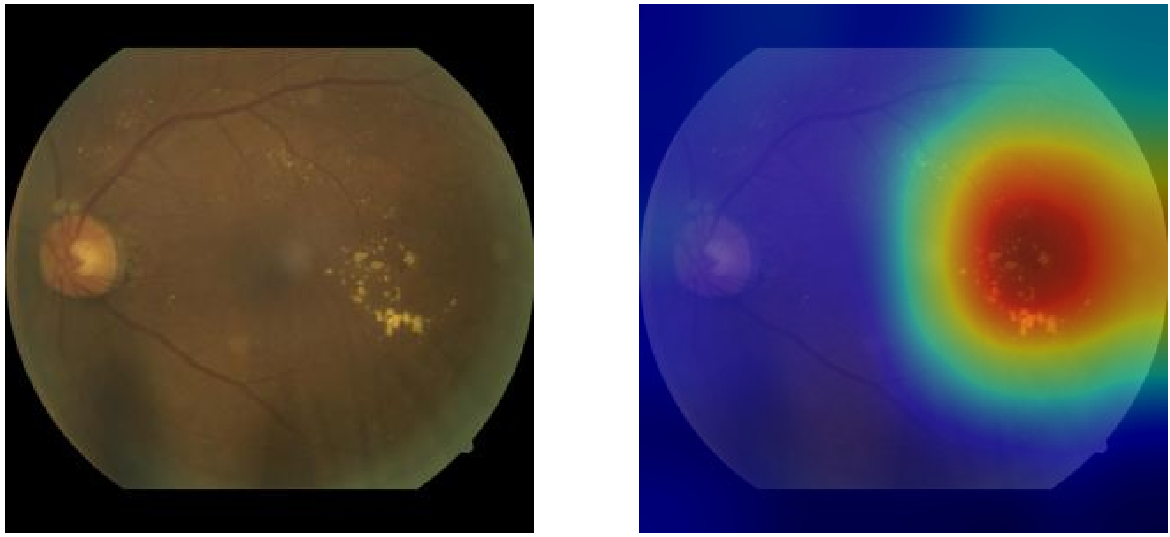
\includegraphics[width=0.75\linewidth]{3.png} \caption{Οπτικοποίηση των περιοχών με DR - Δείγμα 3}
      \label{figure:viz3n}    
  \end{figure}

\begin{figure}[!h]
    \centering
      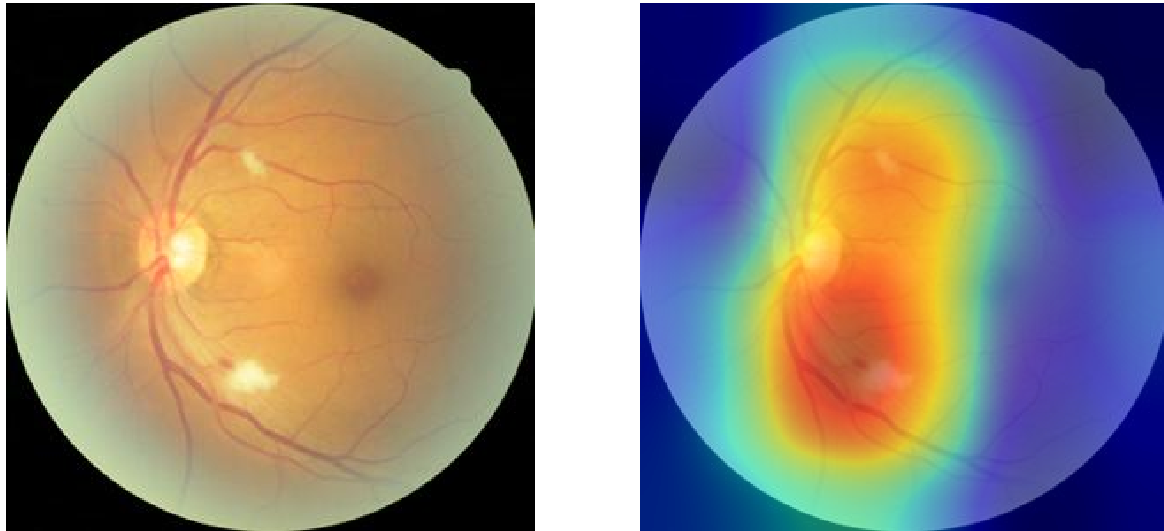
\includegraphics[width=0.75\linewidth]{4.png} \caption{Οπτικοποίηση των περιοχών με DR - Δείγμα 4}
      \label{figure:viz4n}    
  \end{figure}

\section{Αποτελέσματα}
\label{sec:7.2}

Στις εικόνες \ref{figure:rgb1} με \ref{figure:lf1} δίνονται τα αποτελέσματα των πειραμάτων. Σε κάθε πίνακα δίνονται οι μετρικές Ευαισθησία και Εξειδίκευση για τα δύο σύνολα ελέγχου Kaggle και Messidor 2. Οι τιμές έχουν στρογγυλοποιηθεί στο τρίτο δεκαδικό ψηφίο. Υπολογίζονται τρία σημεία για κάθε σύνολο δεδομένων και η μετρική AUC. Τα σημεία που υπολογίζονται είναι το βέλτιστο σημείο(Best Point), το σημείο υψηλής Ευαισθησίας και το σημείο υψηλής Εξειδίκευσης.

Επιλέχθηκε η παρουσίαση 3 σημείων καθώς ανάλογα με την εφαρμογή χρησιμοποίησης του αλγορίθμου θα απαιτούνταν και χρήση διαφορετικού σημείου. Παραδείγματος χάριν, σε ένα μαζικό πρόγραμμα διάγνωσης της rDR που μόνο οι εικόνες των ατόμων που διαγνώστηκαν από τον αλγόριθμο με rDR θα επανεξετάζονταν από ειδικό ιατρό, θα ήταν επιθυμητή η χρήση του σημείου υψηλής Ευαισθησίας. Η επιλογή αυτή θα ήταν θεμιτή καθώς θα ήταν σημαντικότερο να ανιχνευτούν όλοι οι ασθενείς, ακόμα και αν αυτό σημαίνει ανίχνευση με rDR, μη ασθενών. Αντίθετα, σε κάποια κλινική που μετά τη εφαρμογή του αλγορίθμου, όλες οι εικόνες θα παραπέμπονταν σε ειδικό ιατρό για την επιβεβαίωση των αποτελεσμάτων και περαιτέρω διάγνωση, θα ήταν θεμιτή η χρήση του βέλτιστου σημείου ώστε να ταξινομηθούν σωστά όσον το δυνατό περισσότερες εικόνες.


Από τους πινάκες είναι φανερό ότι ο αλγόριθμος παρουσιάζει καλύτερα αποτελέσματα στην ανίχνευση των ατόμων χωρίς rDR. Όπως εξηγήθηκε στην πειραματική διαδικασία οι 2 κλάσεις ήταν αρκετά μη ισορροπημένες, με την κλάση no rDR να παρουσιάζει πάνω από 4 φορές περισσότερα δείγματα. Για αυτό το λόγο κατά την εκπαίδευση έγινε χρήση της κλάσης βάρους ώστε να δίνεται μεγαλύτερη βαρύτητα στις εικόνες με rDR. Ωστόσο, ακόμα και με αυτές τις συνθήκες η ροπή προς την κλάση no rDR είναι εμφανής.

Στα πειράματα παρατηρούνται πολύ καλύτερα αποτελέσματα στο σύνολο δεδομένων Messidor 2 το οποίο είναι αναμενόμενο καθώς όπως αναφέρθηκε, το σύνολο δεδομένων Kaggle αποτελείται από αρκετές μη βαθμολογήσιμες εικόνες λόγω χαμηλής ποιότητας ενώ κάποιες εικόνες έχουν ταξινομηθεί σε λάθος κλάση.

Από τους πίνακες είναι φανερό ότι οι μέθοδοι Ensemble με ψηφοφορία και Ensemble μέσης τιμής έχουν υψηλότερες τιμές AUC έναντι των άλλων μεθόθων και για τα δύο σύνολα δεδομένων. Επιπλέον, φαίνεται να παρουσιάζουν οριακά καλύτερα αποτελέσματα για κάποια σημεία. Για να γίνει πιο εύκολη η σύγκριση των μεθόδων παρουσιάζεται ο συγκεντρωτικός πίνακας \ref{figure:compare1} που συνοψίζει τα αποτελέσματα των πινάκων \ref{figure:rgb1} με \ref{figure:lf1}. Ουσιαστικά για κάθε σημείο έχει αθροιστεί η τιμή της Ευαισθησίας και της Εξειδίκευσης. Με πορτοκαλί έχουν επισημανθεί τα σημεία με τις υψηλότερες τιμές. Γενικά, τα καλύτερα αποτελέσματα δίνονται με το Ensemble μέσης τιμής, έπεται το ensemble με ψηφοφορία ενώ πολύ καλά αποτελέσματα δίνει o SVM με γραμμικό πυρήνα στο σύνολο δεδομένων Messidor 2.

\begin{figure}[!h]
    \centering
      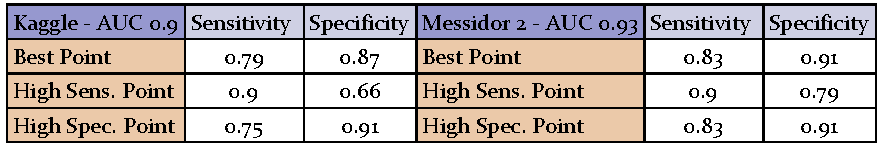
\includegraphics[width=1\linewidth]{rgb1.pdf} \caption{CNN με RGB εικόνες}
      \label{figure:rgb1}    
  \end{figure}
  

\begin{figure}[!h]
    \centering
      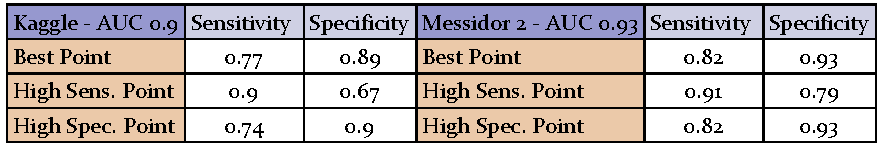
\includegraphics[width=1\linewidth]{linear1.pdf} \caption{CNN και γραμμικός SVM}
      \label{figure:linear1}    
  \end{figure}   
 
  

\begin{figure}[!h]
    \centering
      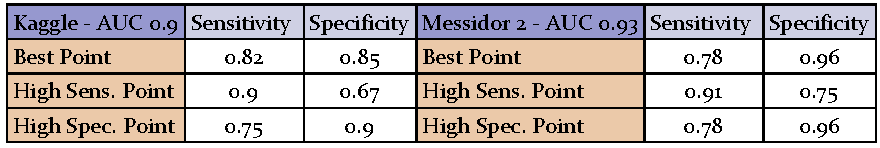
\includegraphics[width=1\linewidth]{rbf1.pdf} \caption{CNN και SVM με RBF πυρήνα}
      \label{figure:rbf1}    
  \end{figure}
  
  
     



\begin{figure}[!h]
    \centering
      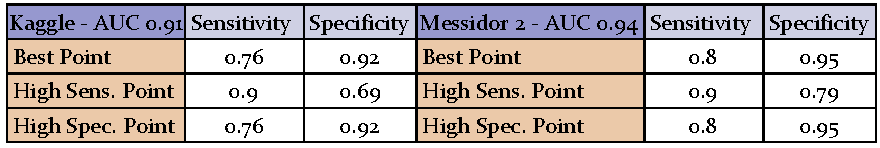
\includegraphics[width=1\linewidth]{ef1.pdf} \caption{Ensemble μέσου όρου με 9 μοντέλων}
      \label{figure:ef1}    
  \end{figure}

\begin{figure}[!h]
    \centering
      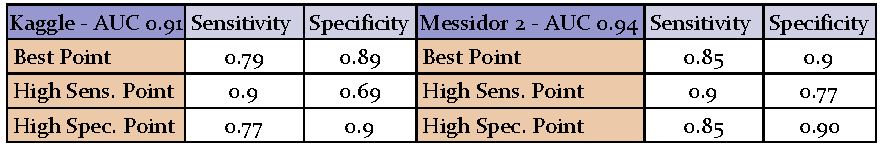
\includegraphics[width=1\linewidth]{lf1.pdf} \caption{Ensemble με ψηφοφορία με 9 μοντέλα}
      \label{figure:lf1}    
  \end{figure}


\begin{figure}[!h]
    \centering
      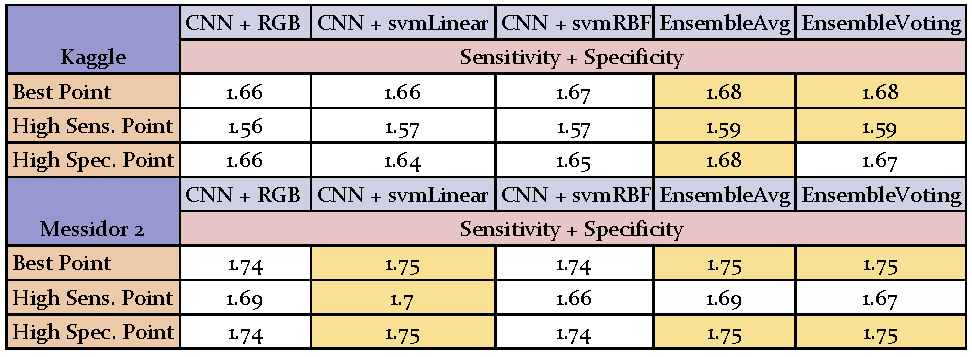
\includegraphics[width=1\linewidth]{compare1.pdf} \caption{Σύγκριση των μεθόδων}
      \label{figure:compare1}    
  \end{figure}





\section{Μελλοντικές Επεκτάσεις}
\label{sec:7.3}

Καθώς το σύνολο δεδομένων που χρησιμοποιήθηκε κατά την εκπαίδευση αποτελείται από χαμηλής ποιότητας εικόνες, μία μελλοντική επέκταση θα αποτελούσε η εφαρμογή όλων των αλγορίθμων που εξετάστηκαν στην παρούσα διπλωματική σε συνδυασμό με ένα νέο σύνολο δεδομένων που θα περιέχει καλύτερης ποιότητας εικόνες.

Επιπλέον, για να επιτευχθούν καλύτερα αποτελέσματα στην οπτικοποίηση των περιοχών με rDR θα μπορούσαν να χρησιμοποιηθούν μεγαλύτερες εικόνες εισόδου ώστε οι χάρτες χαρακτηριστικών του τελευταίου συνελικτικού επιπέδου να έχουν μεγαλύτερες διαστάσεις από 8x8 και έτσι να εντοπίζονται με μεγαλύτερη ακρίβεια τα συμπτώματα της ασθένειας. Επιπλέον, θα ήταν δυνατό να χρησιμοποιηθεί μία διαφορετική αρχιτεκτονική που θα μείωνε λιγότερο τις διαστάσεις της εικόνας στο τελευταίο συνελικτικό επίπεδο. Θεωρητικά μια τέτοια αλλαγή θα μπορούσε να επιφέρει και καλύτερα αποτελέσματα στην ικανότητα πρόβλεψης του μοντέλου.

